\documentclass[10pt,a4paper]{article}
\usepackage[margin=2.1cm]{geometry}
\usepackage{amsmath,amssymb}
\usepackage{booktabs}
\usepackage{graphicx}
\usepackage{float}
\usepackage{caption}
\usepackage{subcaption}
\usepackage{xcolor}
\usepackage{hyperref}
\usepackage{natbib}
\usepackage{microtype}
\usepackage{array}
\usepackage{tabularx}
\usepackage{url}
\graphicspath{{figures/}}
\hypersetup{colorlinks=true,linkcolor=blue,citecolor=blue,urlcolor=blue}
\setlength{\parskip}{0.35em}
\setlength{\parindent}{0pt}
\captionsetup{font=small,labelfont=bf}
\newcommand{\code}[1]{\texttt{#1}}

\title{\vspace{-1.4cm}\textbf{DSA5208 Project 3}\\Parallel K-Means on Covertype: Combined GitHub and Personal Vanda Results}
\author{[Team Member 1: Name, Student ID] \and [Team Member 2: Name, Student ID]}
\date{November 2026}

\begin{document}
\maketitle

\begin{abstract}
We study Lloyd's K-means on the UCI Covertype dataset ($N=581{,}012$,
$D=54$, $K=7$) using serial C++, OpenMP, MPI, hybrid MPI+OpenMP, Apple Metal
and NVIDIA CUDA implementations. The report uses the verified
\code{origin/main} results at commit \code{c450025} only: 27-row MPI strong
and weak campaigns at 256 cores, 21-row 64-core Hybrid layouts, a
five-repetition pinned-core 256$\times$1 Hybrid experiment, 30 CUDA runs and
30 Metal runs. On four 64-core GN-A40 nodes the MPI fit time falls from
2.887~s at one rank to 0.0223~s at 256 ranks (129.7$\times$, 50.7\%
efficiency); weak scaling at 50,000 observations per rank retains 80.2\% at
256 ranks. A separate eight-node 32-core campaign exposes a collective-path
anomaly: its 256-rank collective takes 0.423~s and efficiency falls to 2.6\%.
The unpinned 256-core Hybrid rows are invalid (a 40$\times$ spread for the same
layout); the pinned 256$\times$1 rerun is stable at 0.0223~s and matches the
MPI-only result, identifying process/thread placement as the cause. CUDA is
correct to tolerance but its end-to-end fit is dominated by transfers and CPU
accumulation, not the assignment kernel. On the original data the converged
K-means partition has ARI 0.022 and NMI 0.065 against the seven cover types:
Euclidean K-means on mixed standardized/binary features does not recover the
labels, a result we separate completely from the resampled performance data.
On the personal 10M fixed-total workload, MPI reaches 133.0$\times$ and
52.0\% efficiency at 256 ranks. The final report additionally uses the valid personal Vanda measurements
(E1C 1M/5M/10M, 10M MPI strong, Vanda OpenMP 1--64 threads, 10M Hybrid 64 and
partial 256, and the 8$\times$32 placement rerun). The E2 1-rank recovery completed and is reported as a standalone check; the
E6-256 256$\times$1 and E6-128 backup jobs were still pending at finalization
and are never reported as completed measurements.
\end{abstract}

\section{Introduction}
K-means \citep{lloyd1982,macqueen1967} is a canonical data-mining workload, but its parallel behaviour is
more subtle than the assignment kernel suggests. The assignment step is
embarrassingly parallel over observations; the centroid update is a global
reduction and a barrier. This report asks how far that structure scales on a
real cluster, where the communication and placement costs appear, and whether
hybrid MPI+OpenMP or a GPU improves the end-to-end fit.

The contributions are:
\begin{itemize}
\item a controlled serial and MPI scaling study on Vanda up to 256 CPU cores;
\item a separate 4$\times$64 versus 8$\times$32 topology comparison, reported
      as a hardware/placement observation rather than a node-count law;
\item a repaired Hybrid analysis that separates invalid unpinned runs from a
      valid five-repetition pinned-core experiment;
\item a CUDA A40 evaluation with transfer, kernel, accumulation and end-to-end
      timings kept distinct;
\item a real-data Covertype interpretation using only the original 581,012
      observations.
\end{itemize}

\section{Dataset and preprocessing}
Covertype \citep{blackard1999} contains 581,012 observations, 54 predictive
features and seven forest-cover classes. The first ten features are
quantitative (elevation, aspect, slope, hydrology, road and fire distances,
hillshade); the remaining 44 are binary wilderness and soil indicators. The
class label is column 55 and is excluded from clustering.

The first ten features are z-scored with the population standard deviation;
zero-variance columns map to zero. The 44 binary indicators remain 0/1. The
same transformation, feature order, seed (42) and K-means++ initialization
\citep{arthur2007} are used by every CPU implementation. The class-ordered file
is read with systematic subsets for the serial size sweep, so class
proportions are not distorted by taking the first rows. The resampled
weak-scaling workload repeatedly samples real Covertype rows; it is benchmark
data, not new forest observations.

\section{K-means algorithm}
For observations $x_i\in\mathbb{R}^{D}$ and centroids $c_k$, squared Euclidean
distance is
\begin{equation}
d^2(x_i,c_k)=\sum_{j=1}^{D}(x_{ij}-c_{kj})^2 .
\end{equation}
Assignment selects the nearest centroid, with ties broken by the lowest
cluster id:
\begin{equation}
a_i=\arg\min_{k\in\{0,\ldots,K-1\}} d^2(x_i,c_k).
\end{equation}
For each cluster, the local sums and counts are
\begin{equation}
S_k=\sum_{i:a_i=k}x_i,\qquad n_k=\sum_{i:a_i=k}1,
\end{equation}
and the update is
\begin{equation}
c_k=\begin{cases}S_k/n_k,&n_k>0,\\ c_k,&n_k=0,\end{cases}
\end{equation}
i.e.\ an empty cluster retains its previous centroid. The objective is
\begin{equation}
\mathrm{SSE}=\sum_{i=1}^{N}d^2(x_i,c_{a_i}).
\end{equation}
The measured convergence rule is zero changed labels over the full dataset;
fixed-iteration runs execute exactly $I=30$ iterations for performance
comparability.

\begin{figure}[H]
\centering
\begin{minipage}{0.93\textwidth}
\small
\begin{verbatim}
initialise K centroids by K-means++ (seed 42)
for iter = 1..I:
    zero local sums S_k and counts n_k
    for each local observation x_i:
        a_i = argmin_k ||x_i - c_k||^2      # lowest id breaks ties
        n_{a_i} += 1
        S_{a_i} += x_i
    allreduce S (K*D doubles) and n plus changed count (K+1 uint64)
    for k = 0..K-1:
        if n_k > 0: c_k = S_k / n_k          # empty cluster keeps c_k
    if global changed labels == 0: stop
\end{verbatim}
\end{minipage}
\caption{Parallel Lloyd iteration used by all CPU implementations. The
assignment and local accumulation are local; the two \code{MPI\_Allreduce}
operations are the synchronization points.}
\label{fig:pseudocode}
\end{figure}

\paragraph{Complexity.}
Each iteration evaluates $N K$ distances of dimension $D$, giving
$O(I N K D)$ arithmetic and $O(NKD)$ serial memory traffic when the data are
streamed. The global reduction carries only $K D$ doubles and $K+1$ integers
per rank, so its \emph{volume} is small ($8KD+8(K+1)=3{,}088$ bytes for
$K=7,D=54$), while its \emph{latency} and synchronization cost grow with rank
count. This is why K-means is data-parallel but not embarrassingly parallel:
the assignment is local, the centroid update is global.

\section{Parallelization design}
\subsection{Serial and OpenMP}
The serial kernel fuses assignment, count and sum accumulation in one pass over
the row-major matrix. The OpenMP \citep{dagum1998} kernel parallelizes that pass with
\code{\#pragma omp for schedule(static)}. Every thread owns a private
$K\times D$ sum array and $K$ counts, avoiding atomics and false sharing of the
rank-level arrays. The main thread folds the private arrays in fixed thread-id
order, so a fixed team size gives a deterministic reduction; only after the
fold does the centroid update run.

\subsection{MPI}
The MPI implementation follows the message-passing model \citep{mpiforum2015}. Observations are partitioned into contiguous blocks. With $P$ ranks,
\code{base = N/P} and the first $N\bmod P$ ranks take one extra row. Each rank
computes local sums and counts, then calls two collectives per iteration:
\code{MPI\_Allreduce} of $K D$ doubles for sums and \code{MPI\_Allreduce} of
$K+1$ \code{uint64} values for counts plus the changed-label count. Every rank
receives the same totals and updates the same centroids. The fit time is the
maximum elapsed time across ranks; phase maxima are reported separately and are
never added to claim a total.

\subsection{Hybrid MPI+OpenMP}
The hybrid program uses the MPI decomposition with an OpenMP team inside each
rank. Thread-local arrays are folded into rank-local totals in fixed thread-id
order; the main thread performs both MPI reductions. \code{MPI\_Init\_thread}
requests \code{MPI\_THREAD\_FUNNELED} and the program verifies the provided
level. This is the correct level because only the main thread calls MPI.

At a fixed 64-core budget, the rank/thread layouts trade collective traffic
against OpenMP synchronization. Fewer ranks reduce the number of participants
in each Allreduce, but each rank has a larger OpenMP team and a larger local
fold/barrier. The measured 64-core comparison in Section~\ref{sec:hybrid}
quantifies that trade-off rather than assuming Hybrid should win.

\subsection{GPU design}
The CUDA \citep{nickolls2008} implementation keeps the K-means logic on the host and runs only the
nearest-centroid assignment on the A40. The centroid matrix ($7\times54$
floats) is placed in constant memory. Stage~A re-uploads the observation matrix
every iteration and reads labels back; Stage~B keeps the matrix resident and
re-uploads only centroids. Device arithmetic is float32, while host sums,
counts, centroid updates and the reference implementation remain float64. The
in-process CPU reference uses the same initialization and iteration count, so
GPU label agreement, centroid difference and inertia difference are measured
rather than assumed. Apple Metal follows the same staging on an M1 Pro; it is
reported as a separate platform, not as a Vanda result.

\section{Experimental setup and methodology}
\subsection{Hardware and software}
Table~\ref{tab:hardware} lists the environments. All primary Vanda runs use
GCC 11.4/11.5, OpenMPI 4.1.8 and \code{-O3 -std=c++17 -DNDEBUG}. The Vanda
jobs use PBS Pro; the 4$\times$64 jobs request four 64-core chunks
(\code{select=4:ncpus=64}), the 8$\times$32 jobs eight 32-core chunks, and the
single-node jobs one 64-core chunk. Atlas is included only as historical
cross-platform context.

\begin{table}[H]
\centering\small
\caption{Environments used by the committed results. The 4$\times$64 and
8$\times$32 Vanda jobs differ in node family as well as node count.}
\label{tab:hardware}
\begin{tabular}{llll}
\toprule
Environment & Shape & CPU / device & Toolchain \\
\midrule
Vanda GN-A40 & 4 nodes $\times$ 64 cores & Xeon Platinum 8452Y & GCC 11.5, OpenMPI 4.1.8 \\
Vanda CN & 8 nodes $\times$ 32 cores & Xeon Platinum 8452Y & GCC 11.4, OpenMPI 4.1.8 \\
Vanda IN & 1 node $\times$ 64 cores & Xeon Gold 6438N & GCC 11.4, OpenMPI 4.1.8 \\
Vanda A40 & 1 GPU + host & NVIDIA A40, sm\_86 & CUDA 12.x, GCC 11.5 \\
Atlas (historical) & 1 node $\times$ 96 cores & AMD EPYC 7R13 & GCC 7.3, OpenMPI 4.1.1 \\
Apple M1 Pro & 8 cores + GPU & Apple M1 Pro & Apple clang 21, Metal \\
\bottomrule
\end{tabular}
\end{table}

\subsection{Timing boundaries and repetitions}
\code{fit\_s} covers the Lloyd iteration loop only. Data loading, preprocessing,
K-means++ initialization, row distribution, MPI collectives and final
validation are separate timers. For MPI, \code{fit\_s} is the maximum rank time;
\code{fit\_min\_s} and \code{fit\_imbalance\_s} expose rank skew.
\code{mpi\_reduction\_s} is the wall time of the two Allreduce calls, including
waiting for the slowest rank; it is not pure network transfer and no bandwidth
is derived from it. GPU kernel time is CUDA-event time; upload, readback, CPU
accumulation and full fit are separate.

Every performance point uses the median of three repetitions unless stated.
The pinned-core experiment uses five repetitions. All performance runs use
K=7, D=54, seed=42, $I=30$ fixed iterations. Strong speedup and efficiency use
the one-rank MPI run as baseline:
\begin{equation}
S(P)=\frac{T_{\mathrm{fit}}(1)}{T_{\mathrm{fit}}(P)},\qquad
E(P)=\frac{S(P)}{P}.
\end{equation}
Weak efficiency is
\begin{equation}
E_{\mathrm{weak}}(P)=\frac{T_{\mathrm{fit}}(1,N_0)}
{T_{\mathrm{fit}}(P,P N_0)},\qquad N_0=50{,}000.
\end{equation}
The serial program is a separate reference and is never the MPI speedup
denominator.

\subsection{Result integrity}
The audit in \code{docs/RESULT\_AUDIT\_GITHUB.md} checks expected row counts,
repetitions, rank/thread sets, dataset size, iteration count, compiler, host,
timing fields and label hashes. Byte-identical duplicate CSV files are not
counted twice. The invalid unpinned 256-core Hybrid files are retained as
diagnostic evidence but excluded from every Hybrid performance conclusion.

The final report combines two explicitly separated sources: the GitHub
baseline at \code{c450025} and the personal Vanda campaign at
\code{3ef17dc}. Table~\ref{tab:provenance} records which experiment comes from
which source. Results from different datasets, node families or binding modes
are never merged into one unqualified curve. Recovery jobs submitted on
2026-11-16 are listed separately and are not used as evidence until their CSVs
pass the audit.

\begin{table}[H]
\centering\scriptsize
\caption{Provenance of the results used in this report.}
\label{tab:provenance}
\resizebox{\textwidth}{!}{\begin{tabular}{p{0.25\textwidth}p{0.47\textwidth}p{0.2\textwidth}}
\toprule
Source & Experiments used & Role \\
\midrule
GitHub \code{c450025} &
E1 50k--581k, E2 4$\times$64 and 8$\times$32, E4 64-core, pinned 256$\times$1,
CUDA A40, Metal, Covertype E9 &
Primary baseline \\
Personal \code{3ef17dc} &
E1C 1M/5M/10M, E3 10M strong, E4 weak, E5 OpenMP 1--64,
E6-64 10M, E6-256 partial, E7 8$\times$32 placement &
Supplementary Vanda \\
Recovery jobs &
E2 1-rank 1563234 (complete; not merged), E6-256 256$\times$1 1563235,
E6-128 backup 1563236/1563237 &
Standalone E2 check; E6 pending \\
\bottomrule
\end{tabular}
}
\end{table}

\section{Serial scaling}
Table~\ref{tab:serialN} and Figure~\ref{fig:serial} show the Vanda serial
sweep on one IN-node core. The fitted log-log exponent over
$N=50{,}000\ldots581{,}012$ is \textbf{1.00}, the expected linear growth of
$O(I N K D)$ when $K,D,I$ are fixed. The K sweep at $N=581{,}012$ has exponent
\textbf{0.80}; this is structurally below one because the per-observation sum
over $D$ features does not grow with $K$ while the number of distance
evaluations does. The K-independent work is visible as a non-zero intercept.

\begin{table}[H]
\centering\small
\caption{Serial fit time on Vanda (one core, K=7, D=54, I=30, median of 3).}
\label{tab:serialN}
\begin{tabular}{rrrr}
\toprule
$N$ & $K$ & fit (s) & total (s)\\
\midrule
50,000 & 7 & 0.2876 & 0.9970\\
100,000 & 7 & 0.5831 & 1.3249\\
200,000 & 7 & 1.1728 & 1.9831\\
400,000 & 7 & 2.3240 & 3.2717\\
581,012 & 7 & 3.3807 & 4.4120\\
\bottomrule
\end{tabular}

\end{table}

\begin{table}[H]
\centering\small
\caption{Serial K sweep at N=581,012 (one core, D=54, I=30, median of 3).}
\label{tab:serialK}
\begin{tabular}{rrr}
\toprule
$K$ & fit (s) & total (s)\\
\midrule
2 & 1.3651 & 2.1862\\
4 & 2.1300 & 3.0265\\
7 & 3.3894 & 4.4183\\
10 & 4.7385 & 5.8961\\
16 & 7.1558 & 8.5493\\
\bottomrule
\end{tabular}

\end{table}

\begin{figure}[H]
\centering
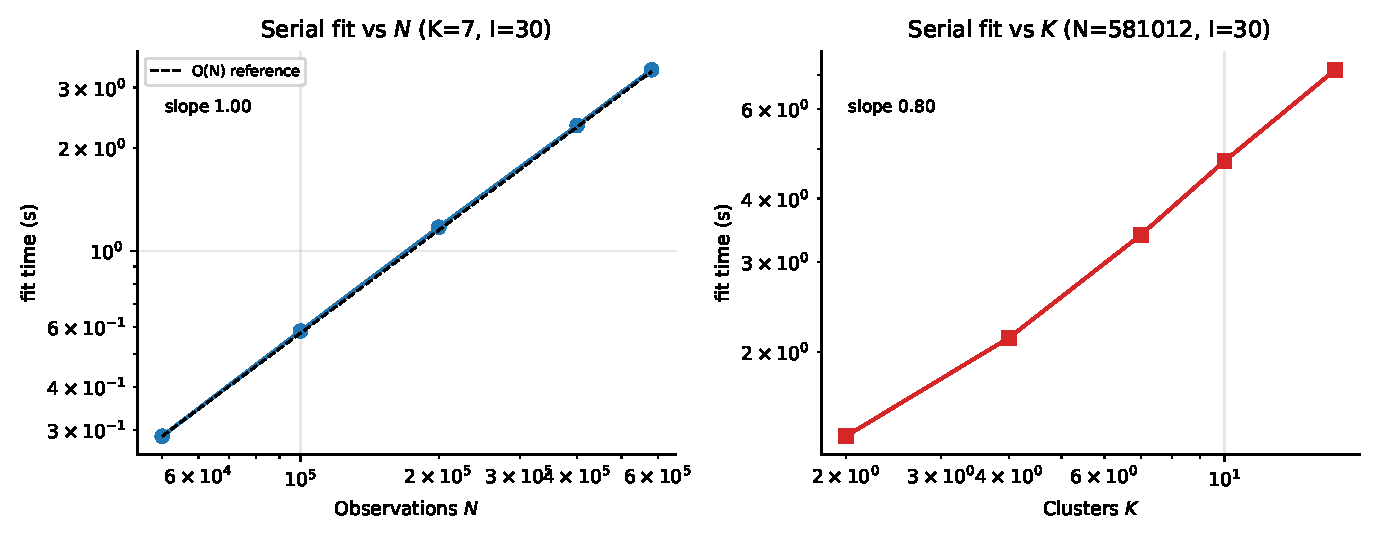
\includegraphics[width=\textwidth]{serial.pdf}
\caption{Serial fit scaling on Vanda. Left: N sweep at K=7; the reference line
is O(N). Right: K sweep at N=581,012. Three repetitions per point.}
\label{fig:serial}
\end{figure}

\subsection{Fixed-total resampled serial extension}
The personal E1C experiment extends the serial baseline to 1M, 5M and 10M
fixed-total resampled observations on one Vanda core (Table~\ref{tab:e1large}).
Fit time grows from 5.42~s at 1M to 54.25~s at 10M, a 10.0$\times$ increase for
a 10$\times$ workload; total time also includes deterministic resampling and
I/O. These points are a separate fixed-total workload and are not merged with
the original-data N sweep.

\begin{table}[H]
\centering\small
\caption{Personal Vanda E1C serial extension, one core, K=7, D=54, I=30,
median of 3.}
\label{tab:e1large}
\begin{tabular}{rrrr}
\toprule
$N$ & fit (s) & total (s) & generation (s)\\
\midrule
1,000,000 & 5.420 & 6.597 & 0.134\\
5,000,000 & 27.072 & 29.414 & 0.668\\
10,000,000 & 54.254 & 58.057 & 1.339\\
\bottomrule
\end{tabular}

\end{table}

\section{MPI strong scaling}
\subsection{Four 64-core nodes}
Table~\ref{tab:strong} and Figure~\ref{fig:strong} show the primary strong
scaling result on four GN-A40 nodes. The one-rank MPI baseline is 2.887~s;
256 ranks reach 0.0223~s, a speedup of \textbf{129.7$\times$} and efficiency
\textbf{50.7\%}. Efficiency remains above 96\% through 16 ranks, then falls to
82.8\% (32 ranks), 78.3\% (64), 60.5\% (128) and 50.7\% (256). At 256 ranks
the per-rank workload is only 2,269 observations, and the two collectives
consume 9.7~ms, 43.7\% of the 22.3~ms fit. The local compute time is 13.3~ms;
the remainder is synchronization and imbalance. This is the expected transition
from computation-dominated to latency-dominated scaling for a small workload.

\begin{table}[H]
\centering\scriptsize
\caption{Vanda MPI strong scaling, N=581,012, K=7, D=54, I=30, 3 repetitions.
The first block is 4$\times$64 GN-A40; the second is 8$\times$32 CN.}
\label{tab:strong}
\resizebox{\textwidth}{!}{\begin{tabular}{llrrrrr}
\toprule
Layout & ranks & fit (s) & speedup & efficiency & collective (s) & collective share\\
\midrule
4$\times$64 & 1 & 2.8874 & 1.00 & 100.0\% & 0.0000 & 0.0\%\\
4$\times$64 & 2 & 1.4547 & 1.98 & 99.2\% & 0.0122 & 0.8\%\\
4$\times$64 & 4 & 0.7253 & 3.98 & 99.5\% & 0.0077 & 1.1\%\\
4$\times$64 & 8 & 0.3663 & 7.88 & 98.5\% & 0.0069 & 1.9\%\\
4$\times$64 & 16 & 0.1863 & 15.50 & 96.9\% & 0.0054 & 2.9\%\\
4$\times$64 & 32 & 0.1090 & 26.49 & 82.8\% & 0.0050 & 4.6\%\\
4$\times$64 & 64 & 0.0576 & 50.14 & 78.3\% & 0.0065 & 11.3\%\\
4$\times$64 & 128 & 0.0373 & 77.49 & 60.5\% & 0.0117 & 31.4\%\\
4$\times$64 & 256 & 0.0223 & 129.73 & 50.7\% & 0.0097 & 43.7\%\\
8$\times$32 & 1 & 2.8827 & 1.00 & 100.0\% & 0.0000 & 0.0\%\\
8$\times$32 & 2 & 1.4558 & 1.98 & 99.0\% & 0.0170 & 1.2\%\\
8$\times$32 & 4 & 1.0230 & 2.82 & 70.4\% & 0.3046 & 29.8\%\\
8$\times$32 & 8 & 0.5695 & 5.06 & 63.3\% & 0.2091 & 36.7\%\\
8$\times$32 & 16 & 0.2922 & 9.87 & 61.7\% & 0.1095 & 37.5\%\\
8$\times$32 & 32 & 0.1488 & 19.37 & 60.5\% & 0.0455 & 30.6\%\\
8$\times$32 & 64 & 0.0868 & 33.22 & 51.9\% & 0.0351 & 40.4\%\\
8$\times$32 & 128 & 0.4259 & 6.77 & 5.3\% & 0.3991 & 93.7\%\\
8$\times$32 & 256 & 0.4374 & 6.59 & 2.6\% & 0.4231 & 96.7\%\\
\bottomrule
\end{tabular}
}
\end{table}

\begin{figure}[H]
\centering
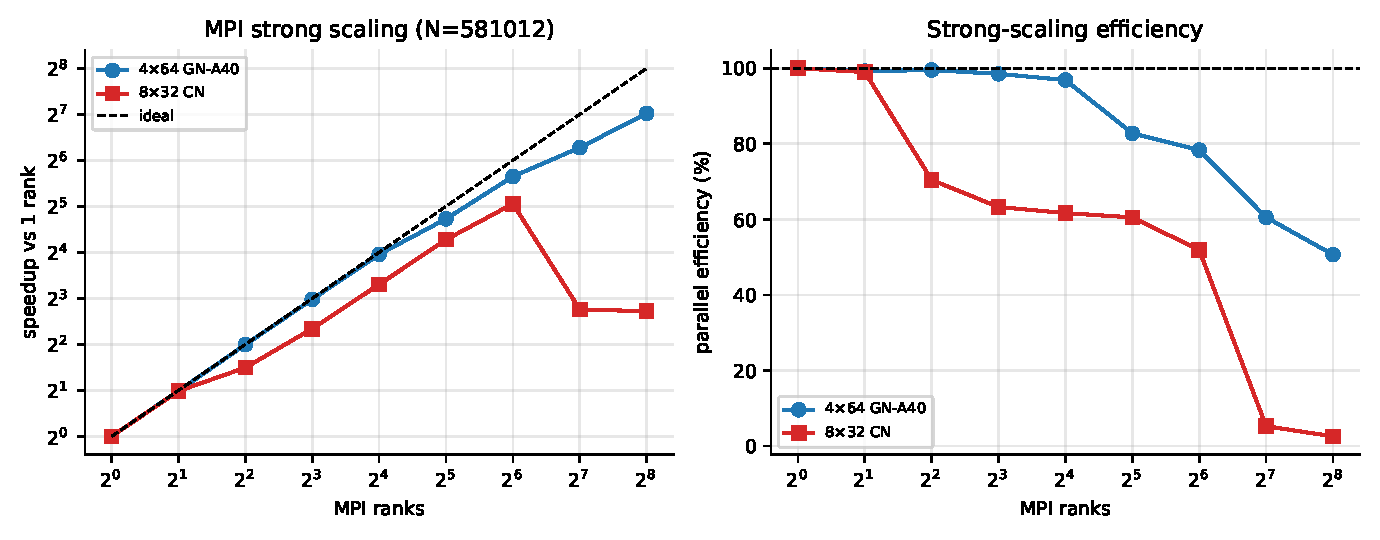
\includegraphics[width=\textwidth]{strong.pdf}
\caption{MPI strong scaling on Vanda. The 8$\times$32 curve is numerically
correct but its collective path collapses at 128--256 ranks; the two layouts
also differ in node family.}
\label{fig:strong}
\end{figure}

\subsection{Eight 32-core nodes and the topology anomaly}
The 8$\times$32 job uses the same CPU model string but a different node family
and node count. Its one-rank baseline is comparable (2.883~s), but from four
ranks onward the collective dominates: 0.305~s at 4 ranks, 0.399~s at 128 and
0.423~s at 256. Speedup collapses to 6.59$\times$ and efficiency to 2.6\% at
256 ranks. Crucially, \code{local\_compute\_s} at 256 ranks is 0.018~s in the
8$\times$32 job versus 0.013~s in the 4$\times$64 job: the arithmetic is not
the problem; the Allreduce is. The two jobs are not a clean 4-versus-8-node
experiment because GN-A40 and CN are different hardware families and the
placement of ranks differs. We therefore report the 8$\times$32 result as a
topology/placement observation, not as evidence that eight nodes are
inherently six times slower. The pinned-core experiment in
Section~\ref{sec:placement} shows that CN nodes can reach 0.0223~s at 256
ranks when placement is controlled.

\subsection{Ten-million-observation strong scaling}
The personal E3 campaign repeats the strong-scaling experiment on the
deterministic fixed-total 10M workload (Table~\ref{tab:e3large},
Figure~\ref{fig:e3large}). One rank takes 49.805~s; 256 ranks take 0.374~s,
a speedup of \textbf{133.0$\times$} and efficiency \textbf{52.0\%}. Up to
16 ranks efficiency is at least 98.7\%, then falls to 85.9\% (32), 67.2\%
(64), 56.2\% (128) and 52.0\% (256). The 10M workload keeps 39,063
observations per rank at 256 ranks, so its efficiency is slightly better than
the 581k workload (50.7\%) at the same rank count, but the collective still
grows from 0.0001~s at one rank to 0.164~s at 256. This is the same
computation-to-communication transition on a larger fixed-total dataset, not a
new scaling law.

\begin{table}[H]
\centering\small
\caption{Personal Vanda 10M fixed-total MPI strong scaling, K=7, D=54, I=30,
3 repetitions. Speedup is relative to one rank.}
\label{tab:e3large}
\begin{tabular}{rrrrr}
\toprule
ranks & fit (s) & speedup & efficiency & collective (s)\\
\midrule
1 & 49.8049 & 1.00 & 100.0\% & 0.0001\\
2 & 24.8786 & 2.00 & 100.1\% & 0.2851\\
4 & 12.4779 & 3.99 & 99.8\% & 0.2270\\
8 & 6.2867 & 7.92 & 99.0\% & 0.1555\\
16 & 3.1544 & 15.79 & 98.7\% & 0.0783\\
32 & 1.8124 & 27.48 & 85.9\% & 0.0568\\
64 & 1.1581 & 43.01 & 67.2\% & 0.3270\\
128 & 0.6923 & 71.94 & 56.2\% & 0.2606\\
256 & 0.3744 & 133.03 & 52.0\% & 0.1638\\
\bottomrule
\end{tabular}

\end{table}

\begin{figure}[H]
\centering
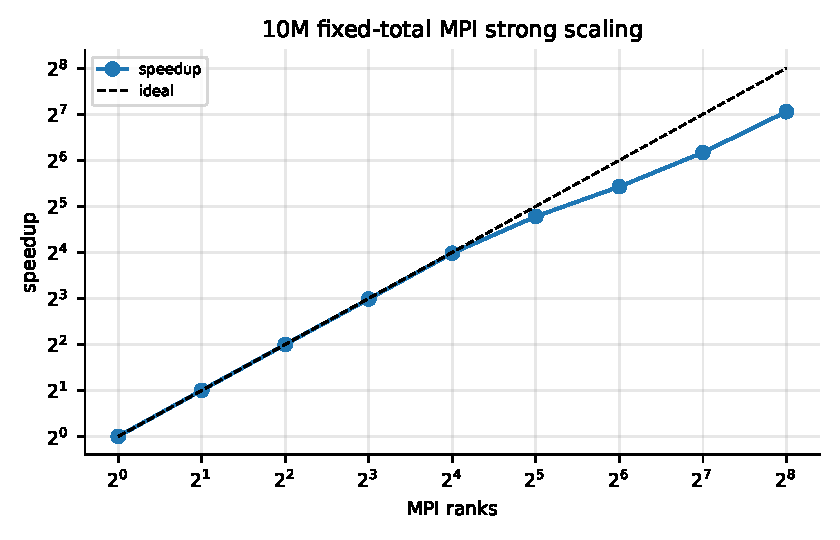
\includegraphics[width=0.68\textwidth]{e3_large.pdf}
\caption{10M fixed-total MPI strong scaling on Vanda. The dashed line is ideal
speedup.}
\label{fig:e3large}
\end{figure}

\section{MPI weak scaling}
Figure~\ref{fig:weak} and Table~\ref{tab:weak} hold the per-rank workload at
50,000 observations while increasing the rank count from 1 to 256; the logical
dataset grows from 50,000 to 12.8 million. On 4$\times$64 the one-rank time is
0.3946~s and the 256-rank time is 0.4922~s, giving weak efficiency
\textbf{80.2\%}. Local compute is essentially constant (0.3945 to 0.4037~s);
the degradation is the collective, which rises from 0.00002~s to 0.2117~s at
256 ranks. On 8$\times$32 the same experiment reaches only \textbf{35.8\%}
because the collective is 0.827~s at 128 ranks and 0.813~s at 256. The
workload is balanced (50,000 observations every rank) and the label hashes
differ across rank counts by design, since each rank count defines a different
logical dataset. Weak efficiency therefore measures communication and
synchronization, not arithmetic imbalance.

\begin{table}[H]
\centering\scriptsize
\caption{Vanda MPI weak scaling, 50,000 observations per rank, K=7, D=54,
I=30, 3 repetitions.}
\label{tab:weak}
\resizebox{\textwidth}{!}{\begin{tabular}{llrrrrr}
\toprule
Layout & ranks & total $N$ & fit (s) & weak eff. & collective (s) & collective share\\
\midrule
4$\times$64 & 1 & 50,000 & 0.3946 & 100.0\% & 0.0000 & 0.0\%\\
4$\times$64 & 2 & 100,000 & 0.3975 & 99.3\% & 0.0039 & 1.0\%\\
4$\times$64 & 4 & 200,000 & 0.3995 & 98.8\% & 0.0084 & 2.1\%\\
4$\times$64 & 8 & 400,000 & 0.4021 & 98.1\% & 0.0092 & 2.3\%\\
4$\times$64 & 16 & 800,000 & 0.4024 & 98.1\% & 0.0109 & 2.7\%\\
4$\times$64 & 32 & 1,600,000 & 0.4062 & 97.1\% & 0.0131 & 3.2\%\\
4$\times$64 & 64 & 3,200,000 & 0.4151 & 95.1\% & 0.0212 & 5.1\%\\
4$\times$64 & 128 & 6,400,000 & 0.4827 & 81.8\% & 0.2019 & 41.8\%\\
4$\times$64 & 256 & 12,800,000 & 0.4922 & 80.2\% & 0.2117 & 43.0\%\\
8$\times$32 & 1 & 50,000 & 0.3916 & 100.0\% & 0.0000 & 0.0\%\\
8$\times$32 & 2 & 100,000 & 0.3976 & 98.5\% & 0.0035 & 0.9\%\\
8$\times$32 & 4 & 200,000 & 0.3969 & 98.6\% & 0.0080 & 2.0\%\\
8$\times$32 & 8 & 400,000 & 0.3979 & 98.4\% & 0.0085 & 2.1\%\\
8$\times$32 & 16 & 800,000 & 0.4010 & 97.6\% & 0.0146 & 3.6\%\\
8$\times$32 & 32 & 1,600,000 & 0.4047 & 96.8\% & 0.1243 & 30.7\%\\
8$\times$32 & 64 & 3,200,000 & 0.4564 & 85.8\% & 0.1755 & 38.4\%\\
8$\times$32 & 128 & 6,400,000 & 1.1078 & 35.3\% & 0.8270 & 74.7\%\\
8$\times$32 & 256 & 12,800,000 & 1.0946 & 35.8\% & 0.8132 & 74.3\%\\
\bottomrule
\end{tabular}
}
\end{table}

\begin{figure}[H]
\centering
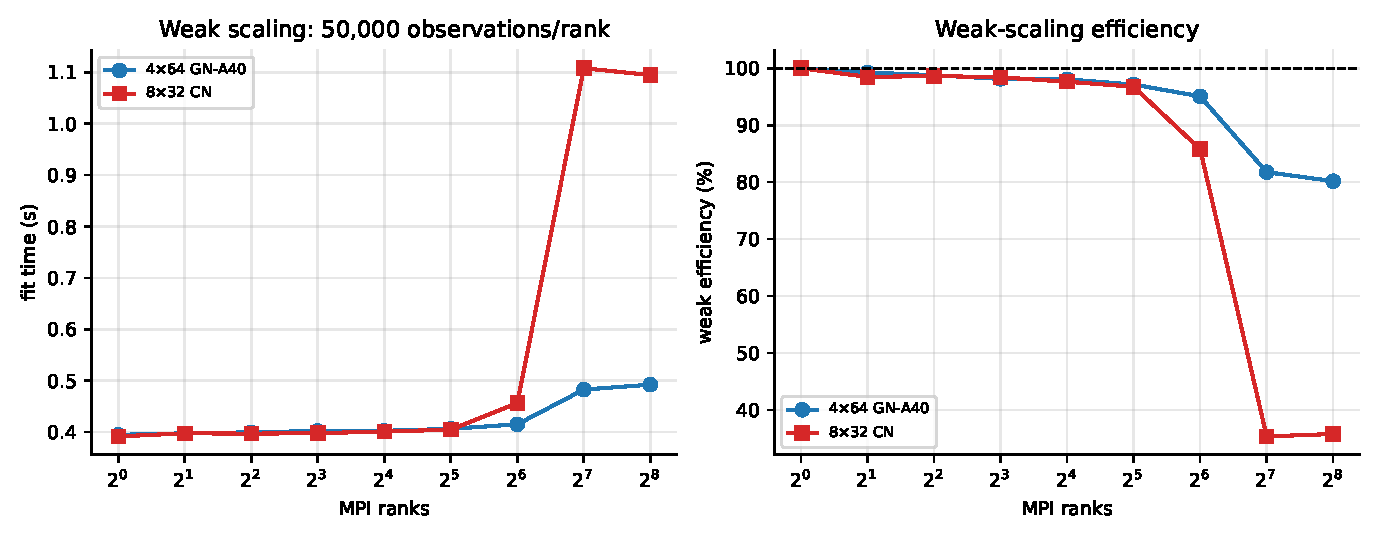
\includegraphics[width=\textwidth]{weak.pdf}
\caption{Weak scaling on Vanda. The 4$\times$64 layout retains 80.2\% at 256
ranks; the 8$\times$32 layout falls to 35.8\% because of collective latency.}
\label{fig:weak}
\end{figure}

\section{OpenMP scaling}
The personal E5 campaign is the primary Vanda OpenMP sweep: one MPI rank on a
single 64-core IN node, with 1--64 threads and three repetitions for both the
original 581,012 data and the 10M fixed-total workload
(Table~\ref{tab:openmpv}, Figure~\ref{fig:openmpv}). On the original data the
fit time falls from 2.530~s at one thread to 0.1045~s at 64 threads
(24.2$\times$); the 10M workload falls from 43.42~s to 1.765~s (24.6$\times$).
Scaling is not monotone at two threads (1.26$\times$ original, 1.41$\times$
10M), which we retain as measured rather than smoothing: the two-thread run is
memory/scheduling limited, while four threads reach 2.58$\times$ on both
datasets. Efficiency at 64 threads is 37.8\% on the original data and 38.4\%
on 10M; the loss is barrier/imbalance and memory bandwidth, not the explicit
thread-local fold, which remains below 0.001~s.

\begin{table}[H]
\centering\small
\caption{Personal Vanda OpenMP scaling, one rank, 1--64 threads, K=7, D=54,
I=30, median of 3. Speedups are relative to one thread.}
\label{tab:openmpv}
\begin{tabular}{rrrrr}
\toprule
threads & original fit (s) & speedup & 10M fit (s) & speedup\\
\midrule
1 & 2.5302 & 1.00 & 43.4167 & 1.00\\
2 & 2.0053 & 1.26 & 30.8255 & 1.41\\
4 & 0.9795 & 2.58 & 16.8540 & 2.58\\
8 & 0.6203 & 4.08 & 8.9654 & 4.84\\
16 & 0.3707 & 6.83 & 4.7963 & 9.05\\
32 & 0.1967 & 12.87 & 3.0350 & 14.31\\
64 & 0.1045 & 24.20 & 1.7652 & 24.60\\
\bottomrule
\end{tabular}

\end{table}

\begin{figure}[H]
\centering
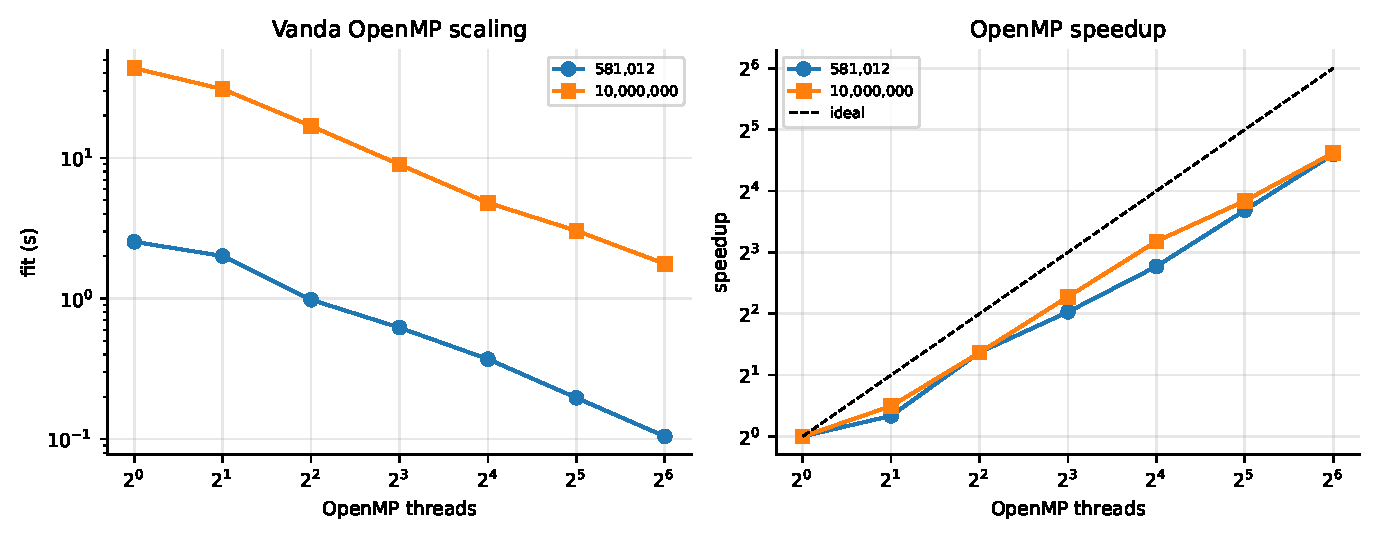
\includegraphics[width=\textwidth]{e5_openmp.pdf}
\caption{Vanda OpenMP fit time and speedup for the original 581,012 data and the
10M fixed-total workload.}
\label{fig:openmpv}
\end{figure}

The earlier Apple M1 Pro 1--4 thread result is not used as a Vanda curve; it is
secondary platform evidence only. The Vanda sweep removes the previous
limitation that no cluster OpenMP-only data existed.

\section{Hybrid MPI+OpenMP}
\label{sec:hybrid}
\subsection{Equal 64-core budgets}
Table~\ref{tab:hybrid64} and Figure~\ref{fig:hybrid64} compare seven layouts
whose ranks $\times$ threads product is exactly 64, on one 64-core IN node.
The MPI-only 64$\times$1 layout is fastest at 0.0779~s. All multi-thread
layouts are slower: 32$\times$2 is 0.0833~s (0.94$\times$ the MPI-only
baseline), 16$\times$4 and 8$\times$8 are 0.0859/0.0856~s, 2$\times$32 is
0.0872~s, and 1$\times$64 is 0.1020~s (0.76$\times$). The phase breakdown
explains why:
\begin{itemize}
\item MPI collective time falls from 0.0259~s at 64$\times$1 to 0.00002~s at
      1$\times$64, as expected when the number of ranks collapses;
\item local compute rises from 0.0736~s to 0.1011~s, because a 64-thread team
      has more synchronization and less efficient per-thread streaming than 64
      independent single-threaded ranks;
\item the explicit OpenMP fold is cheap, rising from 0.000013~s to
      0.000526~s; it is not the dominant cost.
\end{itemize}
The result is a genuine trade-off, not a failure of Hybrid: fewer ranks reduce
collective traffic, but the OpenMP team loses more in local execution than it
saves in communication at this problem size. Hybrid is therefore not assumed
to outperform MPI-only.

\begin{table}[H]
\centering\small
\caption{Hybrid layouts at a fixed 64-core budget, one Vanda IN node,
N=581,012, K=7, D=54, I=30, 3 repetitions. Speedup is relative to
64$\times$1.}
\label{tab:hybrid64}
\resizebox{\textwidth}{!}{\begin{tabular}{rrrrrrr}
\toprule
ranks & threads & fit (s) & speedup vs 64$\times$1 & local (s) & collective (s) & thread reduction (s)\\
\midrule
64 & 1 & 0.0779 & 1.00 & 0.0736 & 0.02590 & 1.30e-05\\
32 & 2 & 0.0833 & 0.94 & 0.0811 & 0.00955 & 2.50e-05\\
16 & 4 & 0.0859 & 0.91 & 0.0831 & 0.00986 & 3.60e-05\\
8 & 8 & 0.0856 & 0.91 & 0.0840 & 0.00613 & 6.00e-05\\
4 & 16 & 0.0853 & 0.91 & 0.0840 & 0.00362 & 1.11e-04\\
2 & 32 & 0.0872 & 0.89 & 0.0865 & 0.00301 & 2.09e-04\\
1 & 64 & 0.1020 & 0.76 & 0.1011 & 0.00002 & 5.26e-04\\
\bottomrule
\end{tabular}
}
\end{table}

\begin{figure}[H]
\centering
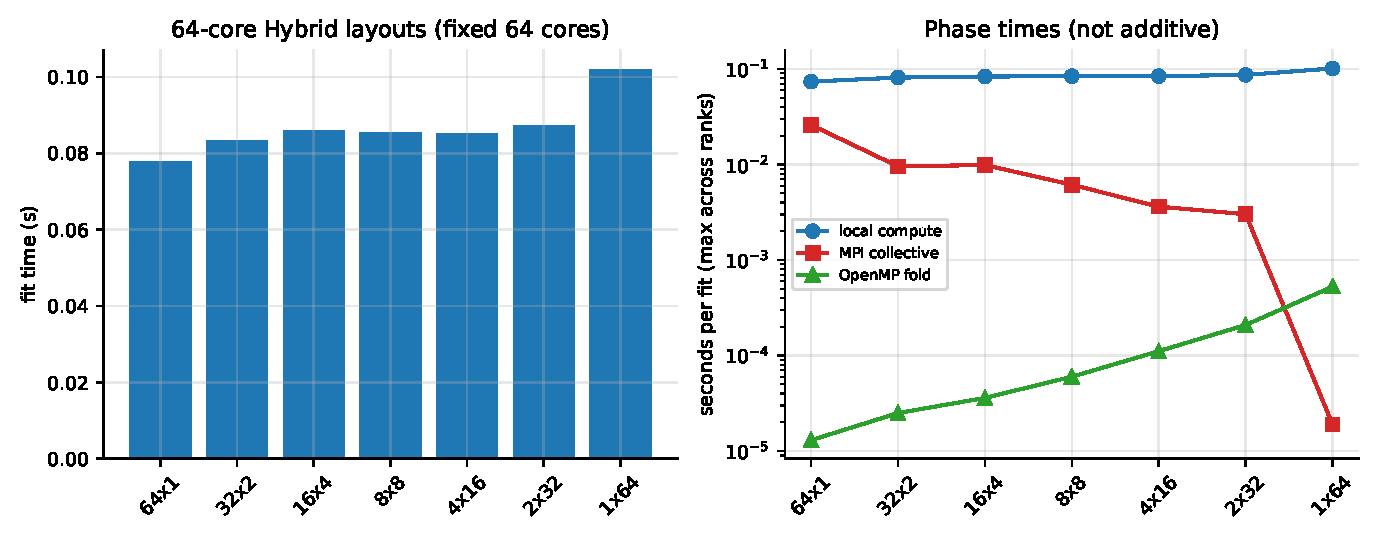
\includegraphics[width=\textwidth]{hybrid64.pdf}
\caption{Left: fit time for seven equal-64-core Hybrid layouts. Right:
phase times; these are maxima across ranks and are not additive, so they are
plotted as separate series rather than stacked.}
\label{fig:hybrid64}
\end{figure}

\subsection{Ten-million-observation Hybrid, 64 and partial 256 cores}
The personal E6 campaign repeats the equal-worker comparison on the 10M
fixed-total workload (Table~\ref{tab:e6ten}, Figure~\ref{fig:e6ten}). At 64
cores the MPI-only 64$\times$1 layout is again fastest at 1.257~s; all
multi-thread layouts are slower (1.404--1.735~s). At the 256-core budget the
backup/original campaign produced six of seven layouts: 128$\times$2 is
0.497~s, 64$\times$4 is 0.489~s, 32$\times$8 is 0.512~s, and the larger
teams are 0.535--0.599~s. The missing 256$\times$1 layout timed out in
preflight and is being recovered as job 1563235; the partial 256-core curve is
therefore shown with an explicit gap, not extrapolated.

\begin{table}[H]
\centering\scriptsize
\caption{Personal Vanda 10M Hybrid, 64-core complete and 256-core partial
(no 256$\times$1). Three repetitions per layout.}
\label{tab:e6ten}
\resizebox{\textwidth}{!}{\begin{tabular}{rrrrrr}
\toprule
budget & ranks & threads & fit (s) & local (s) & collective (s)\\
\midrule
64 & 64 & 1 & 1.2568 & 1.2373 & 0.3669\\
64 & 32 & 2 & 1.5102 & 1.4960 & 0.4551\\
64 & 16 & 4 & 1.4241 & 1.4143 & 0.3143\\
64 & 8 & 8 & 1.4040 & 1.4007 & 0.3056\\
64 & 4 & 16 & 1.5800 & 1.5691 & 0.1842\\
64 & 2 & 32 & 1.5539 & 1.5451 & 0.0275\\
64 & 1 & 64 & 1.7348 & 1.7336 & 0.0001\\
256 & 128 & 2 & 0.4972 & 0.4192 & 0.2629\\
256 & 64 & 4 & 0.4891 & 0.4590 & 0.2203\\
256 & 32 & 8 & 0.5121 & 0.4819 & 0.2183\\
256 & 16 & 16 & 0.5347 & 0.4992 & 0.2193\\
256 & 8 & 32 & 0.5584 & 0.5243 & 0.1084\\
256 & 4 & 64 & 0.5994 & 0.5641 & 0.1583\\
\bottomrule
\end{tabular}
}
\end{table}

\begin{figure}[H]
\centering
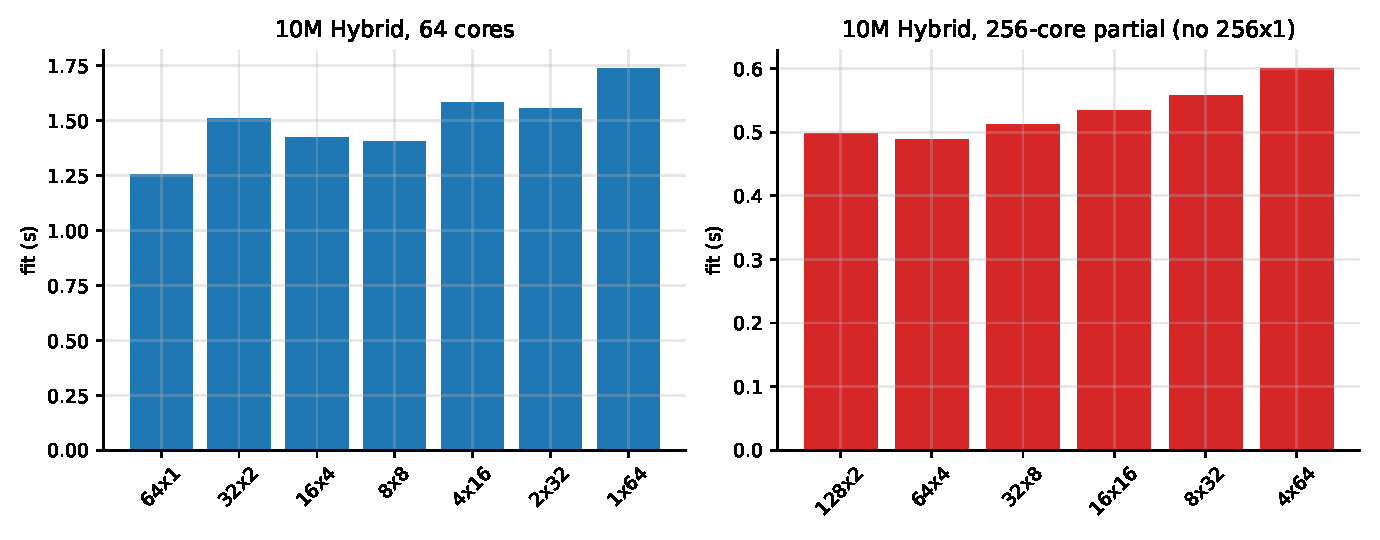
\includegraphics[width=\textwidth]{e6_hybrid_10m.pdf}
\caption{10M Hybrid fit time. Left: complete 64-core layouts. Right: partial
256-core campaign with the missing 256$\times$1 layout explicitly absent.}
\label{fig:e6ten}
\end{figure}

\subsection{256 cores: invalid unpinned runs and the pinned rerun}
\label{sec:placement}
The committed 256-core unpinned Hybrid CSVs are internally inconsistent and
must not be used as performance evidence. For layout 256$\times$1 the three
repetitions are 0.0273, 0.7690 and 1.0875~s, a 40$\times$ spread; the other
layouts are around 1.3--3.0~s, and the measured collective reaches 2.0~s. The
8$\times$32 variant shows the same pattern (0.0365, 0.7746, 0.8044~s for
256$\times$1; 3.4--4.1~s for 8$\times$32). These rows are retained for
diagnosis but excluded from all conclusions.

The later pinned-core experiment reruns only the legal pinned layout,
256$\times$1, on four 64-core CN nodes with \code{--map-by core --bind-to core}
and five repetitions. It gives 0.02208--0.02410~s, median \textbf{0.02227~s},
standard deviation 0.00083~s (CV 3.7\%), and the same label hash as the MPI
runs. This is statistically indistinguishable from the MPI-only 256-rank
4$\times$64 result (0.02226~s) and from the fastest unpinned repetition, while
removing the 40$\times$ variability. The correct interpretation is that the
unpinned failures were a placement/binding problem, not a K-means or fabric
capacity limit. It also shows that CN nodes can deliver 0.022~s at 256 ranks
when placement is controlled; the 8$\times$32 anomaly is therefore not a
simple ``CN hardware is slow'' effect.

\begin{table}[H]
\centering\small
\caption{256-core Hybrid 256$\times$1: MPI-only baseline, pinned rerun and
invalid unpinned run. `--' marks a value not available from the three-rep
summary.}
\label{tab:hybrid256}
\begin{tabular}{lrrrrrr}
\toprule
Configuration & reps & median (s) & min (s) & max (s) & SD (s) & collective (s)\\
\midrule
MPI-only 256 ranks & 3 & 0.0223 & 0.0214 & 0.0281 & -- & 0.0097\\
Hybrid 256$\times$1 pinned & 5 & 0.0223 & 0.0221 & 0.0241 & 0.0008 & 0.0106\\
Hybrid 256$\times$1 unpinned & 3 & 0.7690 & 0.0273 & 1.0875 & 0.5440 & 0.7558\\
\bottomrule
\end{tabular}

\end{table}

\begin{figure}[H]
\centering
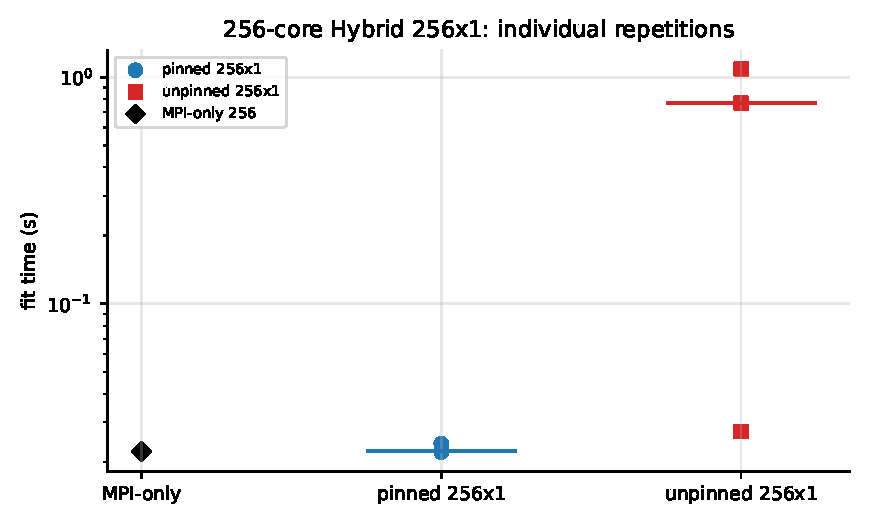
\includegraphics[width=0.66\textwidth]{hybrid256.pdf}
\caption{The pinned 256$\times$1 Hybrid run is stable and matches the MPI-only
fit; the unpinned run spans a 40$\times$ range. Log scale.}
\label{fig:hybrid256}
\end{figure}

The pinned experiment does not validate multi-thread layouts with real
per-rank core reservation: the available launcher hangs for \code{pe=} forms,
and \code{--bind-to core} would pin a whole OpenMP team to one core. The only
correctly pinned Hybrid layout is therefore 256$\times$1, which is effectively
MPI-only. This is a limitation of the placement study, not a reason to treat
the invalid multi-thread rows as valid.

\section{GPU evaluation}
\subsection{NVIDIA CUDA on Vanda}
Table~\ref{tab:cuda} and Figure~\ref{fig:cuda} summarize 30 runs on one A40.
At N=581,012 the assignment kernel takes 0.365~ms, the CPU double-precision
assignment pass takes 89.5~ms, and the full Stage-B fit takes 0.644~s. The
kernel is much faster than the CPU assignment, but the end-to-end fit is
dominated by CPU accumulation (0.613~s) and label readback (0.007~s), not by
the kernel. Stage~A is slower (2.109~s full fit) because it re-uploads the
observation matrix every iteration: 1.492~s of upload time at 581,012. The
Stage-B optimization, keeping the matrix resident, reduces the full fit by
about 3.3$\times$ at the largest size.

Numerical agreement is exact for 50k, 100k, 200k and 581k; at 400k it is
0.9999875 with maximum centroid difference $8.54\times10^{-5}$ and relative
inertia difference $3.2\times10^{-8}$. This is consistent with float32 device
arithmetic against a float64 host reference and is not a correctness failure.
The comparison in the figure is assignment-to-assignment and fit-to-fit; the
0.365~ms kernel time is never presented as a 245$\times$ end-to-end speedup.
The GPU still performs only the assignment; accumulation and centroid update
remain on the CPU, which is the main optimization opportunity.

\begin{table}[H]
\centering\scriptsize
\caption{CUDA A40 medians, 3 repetitions per point. Kernel is CUDA-event
time in milliseconds; all other times are seconds. Agreement is against the
in-process double-precision CPU reference.}
\label{tab:cuda}
\resizebox{\textwidth}{!}{\begin{tabular}{llrrrrrrr}
\toprule
stage & $N$ & fit (s) & kernel (ms) & CPU assign (s) & upload (s) & readback (s) & accumulate (s) & agreement\\
\midrule
A\_assign & 50,000 & 0.0964 & 0.035 & 0.0080 & 0.0706 & 0.0009 & 0.0271 & 1.000000\\
A\_assign & 100,000 & 0.2354 & 0.072 & 0.0162 & 0.1628 & 0.0017 & 0.0742 & 1.000000\\
A\_assign & 200,000 & 0.6939 & 0.132 & 0.0324 & 0.4906 & 0.0030 & 0.2023 & 1.000000\\
A\_assign & 400,000 & 1.4238 & 0.253 & 0.0635 & 1.0025 & 0.0056 & 0.4262 & 0.999988\\
A\_assign & 581,012 & 2.1088 & 0.362 & 0.0895 & 1.4923 & 0.0076 & 0.6218 & 1.000000\\
B\_full & 50,000 & 0.0301 & 0.035 & 0.0081 & 0.0046 & 0.0012 & 0.0270 & 1.000000\\
B\_full & 100,000 & 0.0600 & 0.071 & 0.0162 & 0.0083 & 0.0021 & 0.0541 & 1.000000\\
B\_full & 200,000 & 0.1851 & 0.132 & 0.0324 & 0.0175 & 0.0039 & 0.1723 & 1.000000\\
B\_full & 400,000 & 0.4326 & 0.252 & 0.0633 & 0.0336 & 0.0056 & 0.4104 & 0.999988\\
B\_full & 581,012 & 0.6444 & 0.365 & 0.0895 & 0.0495 & 0.0070 & 0.6129 & 1.000000\\
\bottomrule
\end{tabular}
}
\end{table}

\begin{figure}[H]
\centering
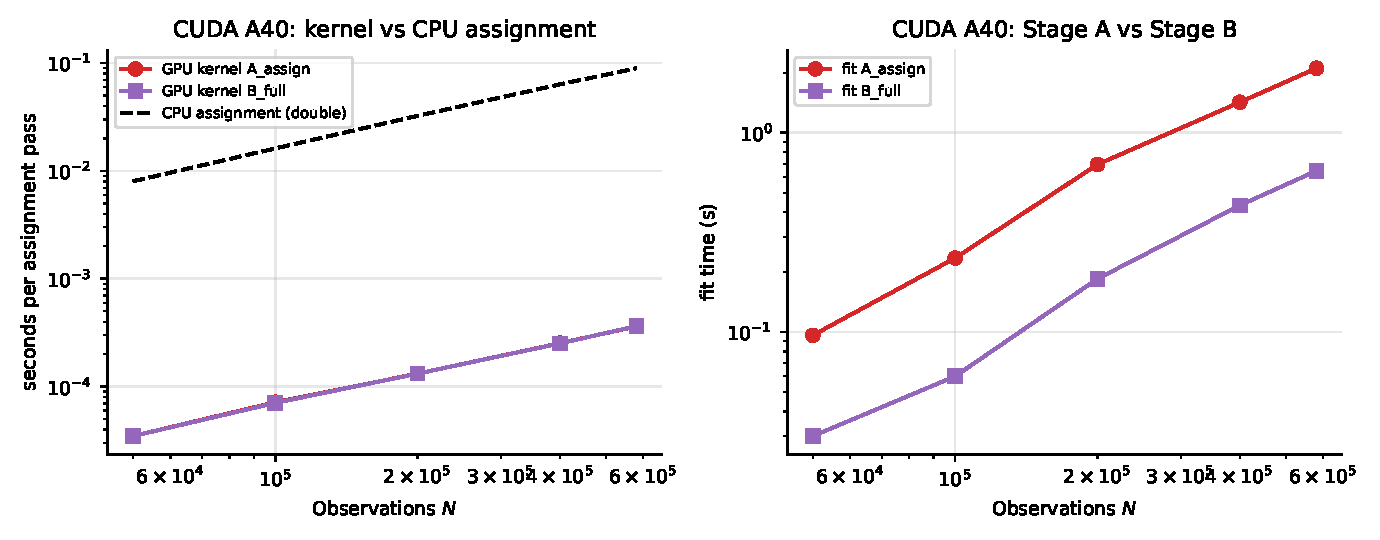
\includegraphics[width=\textwidth]{cuda.pdf}
\caption{CUDA A40. Left: assignment kernel versus a CPU double-precision
assignment pass. Right: full Stage-A and Stage-B fit times. Kernel time is not
compared with CPU end-to-end time.}
\label{fig:cuda}
\end{figure}

\subsection{Apple Metal (separate platform)}
The Metal implementation on an M1 Pro agrees with the CPU labels at every
measured size (20k--400k) and has label agreement 1.0. At 400k the Stage-A fit
is 0.915~s, Stage-B is 0.673~s, the GPU kernel is 0.020~s and the CPU
assignment is 0.079~s. The same caveat applies: the kernel is faster than the
CPU assignment, but neither GPU stage beats the best CPU implementation
end-to-end, and the hardware is not Vanda. Metal is reported only as a
secondary GPU portability result.

\begin{figure}[H]
\centering
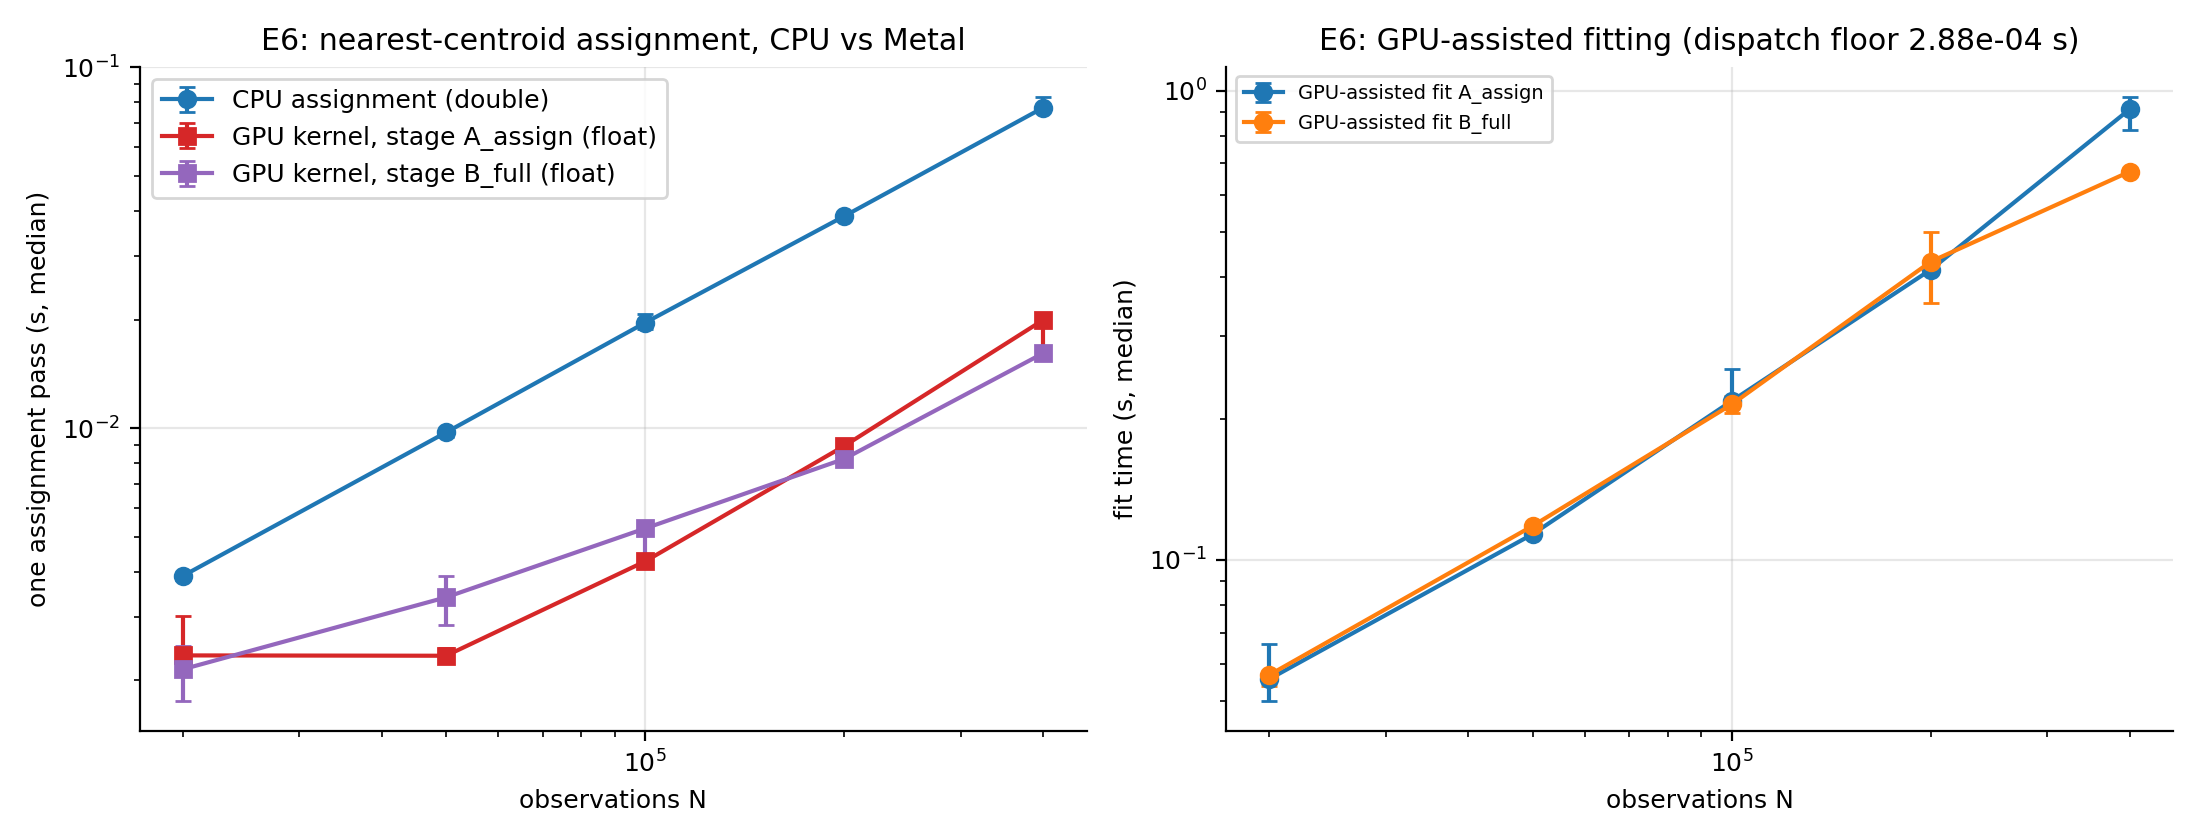
\includegraphics[width=0.92\textwidth]{metal.png}
\caption{Apple Metal evaluation on an M1 Pro. This is a separate platform
from the Vanda CPU/CUDA results and is not mixed into a scaling curve.}
\label{fig:metal}
\end{figure}

\section{Communication, affinity and additional experiments}
Figure~\ref{fig:comm} isolates the collective behaviour. On 4$\times$64 the
Allreduce is 5--12~ms and its share is below 5\% until 64 ranks, then rises to
31\% at 128 and 44\% at 256. On 8$\times$32 the collective is already 30\% at
four ranks, 94\% at 128 and 97\% at 256. The K-means payload is only 3,088
bytes per rank per iteration, so this is latency and placement, not bandwidth.
The timing includes waiting for slower ranks; it is not pure network transfer.

\begin{figure}[H]
\centering
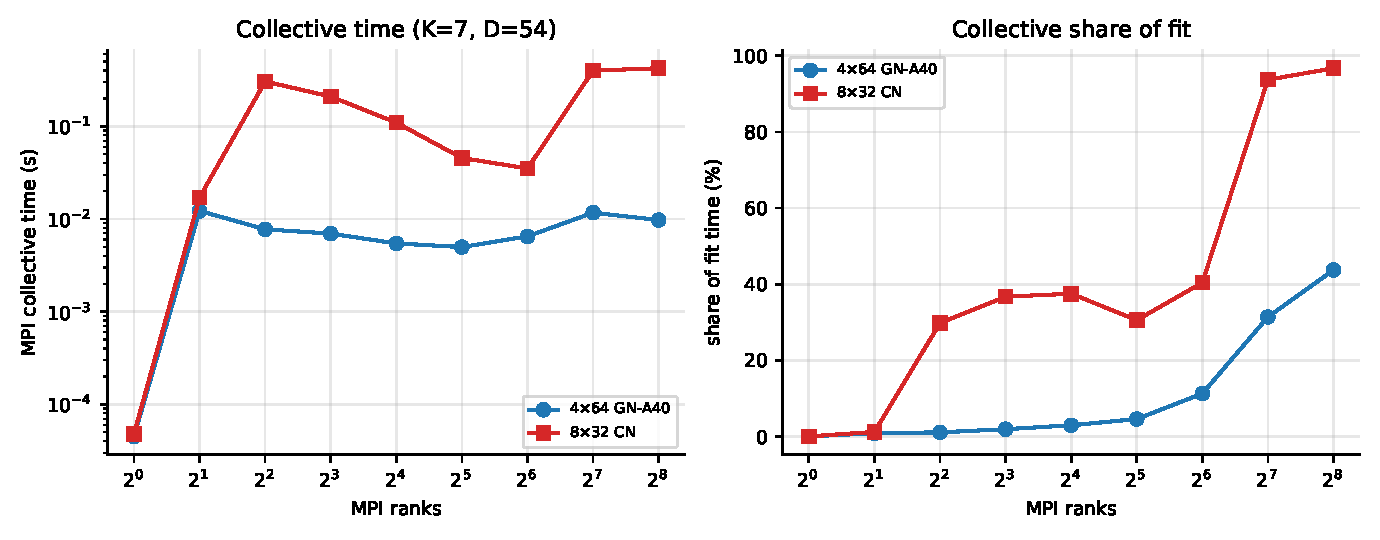
\includegraphics[width=\textwidth]{communication.pdf}
\caption{MPI collective time and its share of fit. The 8$\times$32 anomaly is
a topology/placement observation; the 4$\times$64 and 8$\times$32 jobs also
use different node families.}
\label{fig:comm}
\end{figure}

\subsection{Personal E7 8$\times$32 placement rerun}
The personal E7 campaign reruns the 8$\times$32 layout at 128 and 256 ranks
(Table~\ref{tab:e7}). At 256 ranks, \code{core}, \code{ppr32} and the
16-ranks-per-node mapping take 0.526, 0.480 and (at 128 ranks) 0.332~s; the
collective accounts for 0.514, 0.467 and 0.307~s respectively. The
8$\times$32 collective anomaly is therefore reproducible under multiple
mappings. The \code{core} and \code{ppr32} logs do not contain the host
placement printout (only \code{ppr16} does), so the result is classified
COMPLETE for timing but LIMITED for placement diagnostics. This is not a clean
node-count comparison: the 8$\times$32 CN layout is a different hardware and
collective path from the 4$\times$64 GN-A40 baseline.

\begin{table}[H]
\centering\small
\caption{Personal E7 8$\times$32 placement rerun, 581,012 original data,
K=7, D=54, I=30, two repetitions per point.}
\label{tab:e7}
\begin{tabular}{llrrr}
\toprule
mapping & ranks & fit (s) & collective (s) & local (s)\\
\midrule
core & 128 & 0.1509 & 0.1257 & 0.0429\\
core & 256 & 0.5262 & 0.5136 & 0.0181\\
ppr32 & 128 & 0.1684 & 0.1432 & 0.0602\\
ppr32 & 256 & 0.4800 & 0.4668 & 0.0182\\
ppr16 & 128 & 0.3323 & 0.3070 & 0.0385\\
\bottomrule
\end{tabular}

\end{table}

\paragraph{Pinned-core experiment.}
The latest measured additional experiment is the five-repetition pinned
256$\times$1 Hybrid run described in Section~\ref{sec:placement}. Its research
question is explicit in the committed script: the unpinned 256$\times$1 fit
varied from 0.027 to 1.088~s, while the pinned K-means phase timers were small
and stable. The corrected run pins every rank to a core on four 64-core CN
nodes and produces 0.0221--0.0241~s, CV 3.7\%. This supports the placement
explanation, but it does not prove which of binding, NUMA placement or
competing OpenMP threads caused the unpinned values; the experiment controls
binding only and uses one thread per rank.

\paragraph{Allreduce microbenchmark (incomplete).}
\path{tests/allreduce_micro.cpp} and \path{jobs/vanda/allreduce_probe.pbs}
are committed to isolate the exact 3,088-byte payload with pinned/unpinned
ranks and competing OpenMP threads. Their research question is the right one,
but \textbf{no output CSV or log is committed}. The probe is therefore
classified INCOMPLETE/UNVERIFIED and no Allreduce-microbenchmark number is
reported. The K-means phase timers remain the measured communication evidence.

\section{Correctness validation}
The repository's test suite compares serial, OpenMP, MPI and Hybrid results on
a synthetic mixture, real Covertype, K=1 and K=7, uneven partitions, more ranks
than observations, fixed-iteration and convergence stopping, and the
empty-cluster policy. The measured performance files provide independent
cross-rank evidence:
\begin{itemize}
\item E2 4$\times$64: every rank count from 1 to 256 produces the same label
      hash \code{15912193932519828622}; the scaling difference is therefore not
      a different clustering.
\item E2 8$\times$32: the same single hash, so its anomaly is communication,
      not numerical divergence.
\item E4 64-core: all seven layouts share one hash; the pinned 256$\times$1
      run also has that hash.
\item Personal E5 and E6: every complete layout has one label hash; the E6-256
      partial rows (128$\times$2 to 4$\times$64) also share it.
\item Personal E3 10M: all rank counts share one hash, so the 133$\times$
      speedup is not a different clustering.
\item CUDA: label agreement 1.0 for all but 400k (0.9999875), maximum centroid
      difference $8.54\times10^{-5}$ and relative inertia difference
      $3.2\times10^{-8}$; Metal agreement is 1.0.
\end{itemize}
Floating-point reductions are not required to be bitwise equal: sums over
different rank/thread orders differ in the last bits. The acceptance criterion
is exact label/cluster-size agreement and tolerance-based centroid/inertia
agreement, with any differing clustering treated as a failure to explain.

The original-data convergence run used for Section~\ref{sec:realdata} ran 91
iterations and converged. It is an analysis run from the GitHub baseline
serial binary and data, not a personal HPC result and not a fixed-iteration
benchmark.

\section{Real-data Covertype interpretation}
\label{sec:realdata}
The performance workloads are resampled and must not be interpreted as new
forest records. For the real-data interpretation we use only the original
581,012 observations. A converged serial run (91 iterations) gives inertia
\textbf{3,712,497.96} and the cluster sizes in Table~\ref{tab:covertype}.
Against the seven known cover types, \textbf{ARI = 0.0220}, \textbf{NMI =
0.0650} and \textbf{AMI = 0.0649}.

\begin{table}[H]
\centering\small
\caption{Converged original-Covertype clusters. Elevation, road distance and
fire distance are inverse-transformed means in the original units.}
\label{tab:covertype}
\resizebox{\textwidth}{!}{\begin{tabular}{rrrrrrrr}
\toprule
cluster & size & share & majority type & purity & elevation & road dist. & fire dist.\\
\midrule
0 & 77,764 & 13.4\% & 1 & 0.500 & 3110 & 4352 & 2103\\
1 & 56,307 & 9.7\% & 2 & 0.445 & 3179 & 2217 & 1880\\
2 & 50,440 & 8.7\% & 2 & 0.404 & 2680 & 1477 & 1287\\
3 & 51,673 & 8.9\% & 2 & 0.712 & 2925 & 3764 & 5070\\
4 & 125,172 & 21.5\% & 1 & 0.462 & 3053 & 2472 & 1560\\
5 & 66,197 & 11.4\% & 2 & 0.411 & 2793 & 1485 & 1473\\
6 & 153,459 & 26.4\% & 2 & 0.538 & 2901 & 1469 & 1704\\
\bottomrule
\end{tabular}
}
\end{table}

\begin{figure}[H]
\centering
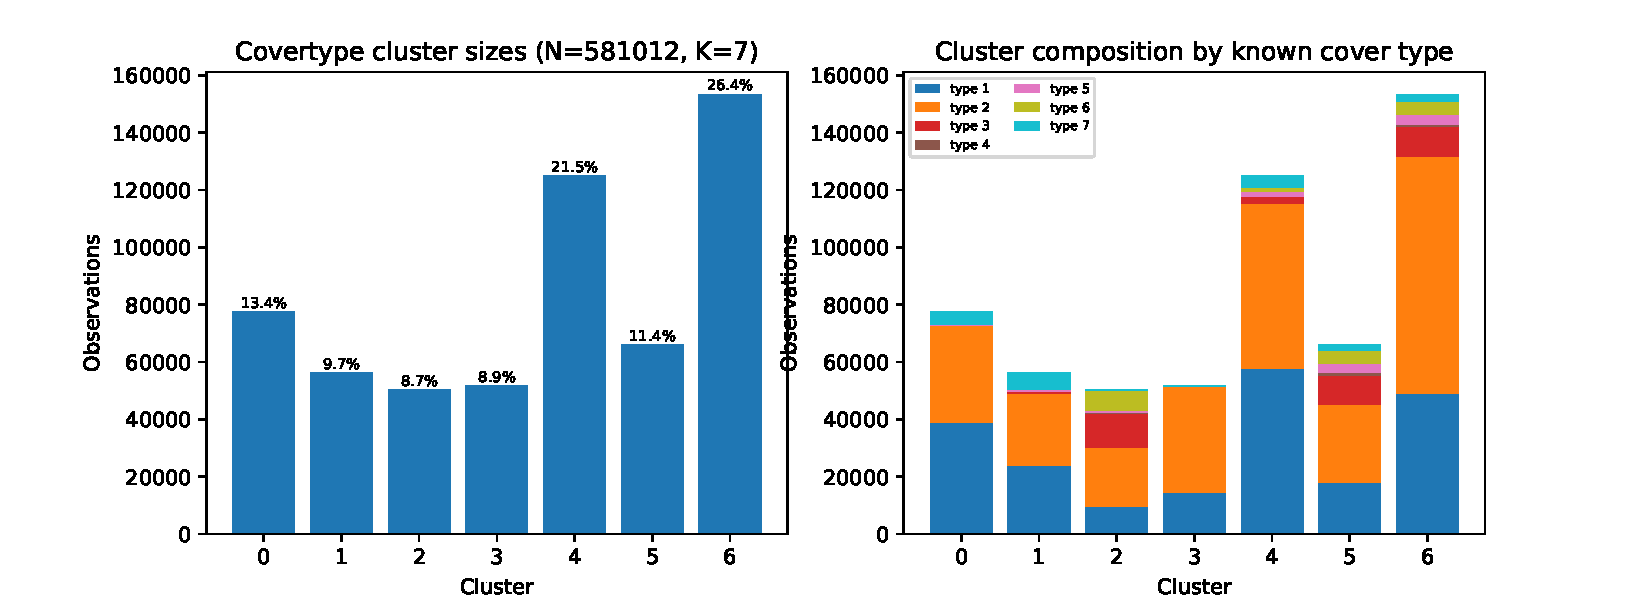
\includegraphics[width=\textwidth]{covertype_clusters.pdf}
\caption{Real-data Covertype cluster sizes and cover-type composition, K=7,
original 581,012 observations. This is separate from all resampled performance
data.}
\label{fig:covertype}
\end{figure}

\begin{figure}[H]
\centering
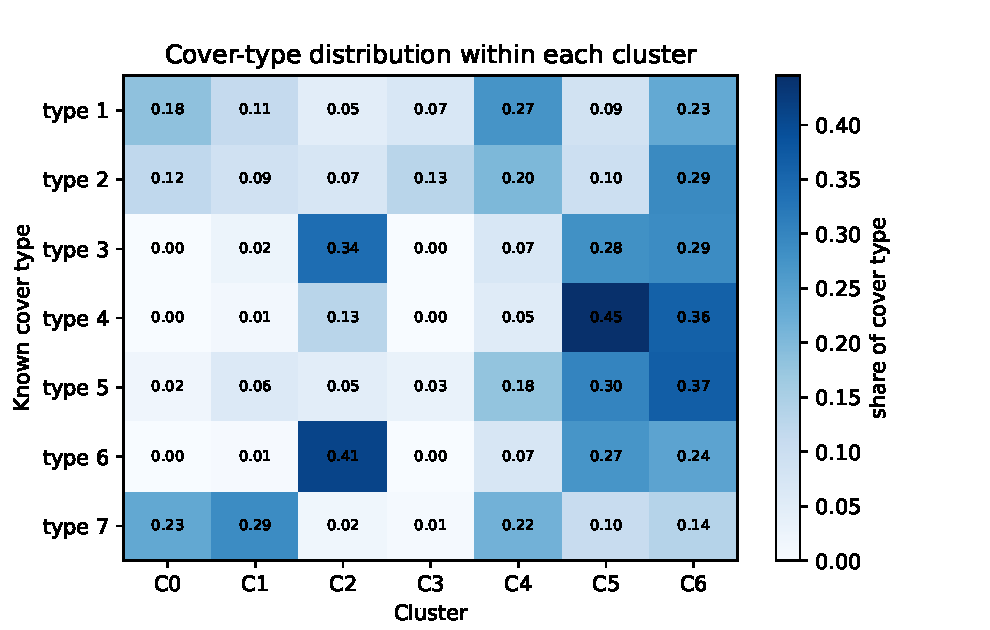
\includegraphics[width=0.72\textwidth]{covertype_contingency.pdf}
\caption{Row-normalized cover-type distribution within each cluster.}
\label{fig:covertype-cont}
\end{figure}

The clusters are not the seven cover types. Every cluster is a mixture,
and the two dominant classes (Lodgepole Pine, 283,301 observations, and
Spruce/Fir, 211,840) occupy most of every cluster. Cluster~3 is the purest
(71.2\% type 2), with the largest mean fire distance (5,070) and a high
elevation (2,925); cluster~0 is 50.0\% type 1 with a large mean road distance
(4,352); clusters~2 and~5 are lower-elevation, steeper-slope groups with more
type 3/6 observations; cluster~4 is the largest (125,172) and 46.2\% type 1.
Rare types are split rather than recovered: 45\% of type-4 observations fall
in cluster~5 and 34\% of type-3 observations fall in cluster~2, but those
clusters remain majority types 1/2.

The low ARI/NMI has a clear explanation. Euclidean K-means on ten standardized
continuous features plus 44 binary indicators is dominated by the high-variance
continuous dimensions and by the binary soil/wilderness patterns; the binary
features are not weighted, and the class imbalance lets the two large classes
dominate the centroid means. K=7 is a modelling choice matching the number of
labels, not a guarantee that the label geometry is seven well-separated
Euclidean clusters. This is a real-data conclusion about the clustering, not a
performance claim, and no resampled workload enters it.

\section{Discussion and limitations}
\paragraph{Why efficiency falls.}
Amdahl's argument \citep{amdahl1967} and its scaled counterpart \citep{gustafson1988} frame the expected limit: at fixed N, increasing P reduces per-rank work while the two collectives remain
per-iteration barriers. On the 581k workload, 256 ranks hold only 2,269
observations each; the 3 KB Allreduce is latency-bound and consumes 44\% of
the fit on the good layout. The 10M-equivalent weak workload keeps 50,000
observations/rank and retains 80.2\% on 4$\times$64, showing that a larger
per-rank workload amortizes the collective. This is the expected
compute-to-communication trade-off, not a defect in the algorithm.

\paragraph{Node layout versus hardware.}
The 4$\times$64 and 8$\times$32 campaigns are not a controlled node-count
experiment: GN-A40 and CN are different node families, and the 8$\times$32
collective collapses by an order of magnitude while local compute stays
similar. The correct conclusion is that the 8$\times$32 configuration in this
campaign suffered a collective/placement problem. The pinned 256$\times$1 run
on four CN nodes reaches the MPI-only time, showing that the CN hardware can
perform well under binding; it does not isolate node count from fabric.

\paragraph{Hybrid trade-offs.}
At 64 cores, MPI-only 64$\times$1 is 24\% faster than 1$\times$64 (0.0779 vs
0.1020~s). The collective share falls as the rank count falls, but local
compute becomes slower with large OpenMP teams; the explicit fold is cheap
(0.5~ms at 64 threads), so the loss is not the fold alone. Hybrid should be
selected only when the communication saving outweighs the OpenMP scheduling
cost, and only with verified affinity. The pinned 256$\times$1 result is
effectively MPI-only and should not be presented as evidence that multi-thread
Hybrid scales.

\paragraph{GPU trade-offs.}
The A40 kernel is far faster than the CPU assignment, but Stage-B still spends
0.613~s in CPU accumulation and 0.007~s in readback at 581k, versus 0.365~ms
in the kernel. A GPU-resident accumulation/centroid update, or a fused
reduction, is the obvious next step. A kernel-only comparison would be
misleading and is deliberately avoided.

\paragraph{Limitations.}
(i) The Vanda OpenMP sweep covers 1--64 threads; 128--256 thread teams were not
measured. (ii) The unpinned 256-core Hybrid rows are invalid and only the
single-thread pinned layout was validated; multi-thread pinned Hybrid is
blocked by the available launcher. (iii) The Allreduce microbenchmark was
committed without results. (iv) The 4$\times$64 and 8$\times$32 layouts are
hardware-confounded. (v) GPU results use one A40 and float32 device arithmetic;
Metal is a different platform. (vi) The real-data analysis is a deterministic
single-seed K-means result, not a statistical guarantee over initializations.
(vii) Serial data cover up to 10M in the fixed-total E1C extension, but no
larger original-data serial baseline exists. (viii) E2 is 24/27 rows (no 1-rank
baseline), E6-256 is 18/21 rows (no 256$\times$1), and E6-128 is still queued;
the recovery/backup jobs in Table~\ref{tab:recovery} were submitted but had no
validated results at finalization.

\section{Recovery status at report finalization}
Four targeted jobs were accepted by PBS on 2026-11-16. The E2 1-rank recovery
1563234 completed with exit 0 and produced three rows (median 3.429~s, same
label hash as the MPI campaign). It ran on one IN-010 node with binding
disabled, while the original E2 campaign ran on a mixed CN/GN allocation;
because the node family differs, the recovery is valid standalone but is not
silently spliced into the 4$\times$64 speedup curve. The E6-256 recovery
1563235 and the E6-128 backup smoke 1563236 were still queued at finalization;
the production backup 1563237 is held behind `afterok:1563236`. The original
E6-128 job 1557221 remains queued and is not cancelled or modified.

\begin{table}[H]
\centering\small
\caption{PBS recovery/backup jobs submitted before report finalization.}
\label{tab:recovery}
\begin{tabular}{lllll}
\toprule
Experiment & Job & Resource & State & Dependency\\
\midrule
E2 1-rank recovery & 1563234 & 1 core & complete, exit 0 & none\\
E6-256 256$\times$1 recovery & 1563235 & 4$\times$64 & queued & none\\
E6-128 backup smoke & 1563236 & 2$\times$64 & queued & none\\
E6-128 backup production & 1563237 & 2$\times$64 & held & afterok:1563236\\
\bottomrule
\end{tabular}

\end{table}

\section{Conclusion}
The GitHub baseline supports a coherent scaling story. MPI strong scaling on
four 64-core GN-A40 nodes reaches 129.7$\times$ and 50.7\% at 256 ranks for the
581k workload, while weak scaling at 50,000 observations/rank retains 80.2\%.
The limiting cost at high rank count is the per-iteration Allreduce, not local
arithmetic. The 8$\times$32 experiment exposes a severe collective/placement
anomaly that must not be reported as a clean node-count result. On the
personal 10M fixed-total workload, MPI reaches 133.0$\times$ and 52.0\% at 256
ranks; the Vanda OpenMP sweep reaches 24.2$\times$ at 64 threads on the
original data. At 64 cores, MPI-only is faster than every equal-core Hybrid
layout; the OpenMP fold is cheap, but large teams lose local efficiency. The pinned 256$\times$1 rerun is
stable and matches MPI-only, confirming that the earlier 40$\times$ spread was
a binding/placement failure. CUDA is numerically sound to float32 tolerance,
but transfer and CPU accumulation dominate end-to-end time. On the original
data, Euclidean K-means does not recover the seven cover types (ARI 0.022,
NMI 0.065); the clusters are mixed, class-imbalanced partitions of the
standardized/binary feature space.

\section{Reproducibility}
The combined report uses the GitHub baseline \code{c450025} plus the personal
branch \code{3ef17dc}. Build:
\begin{verbatim}
make cpu          # serial, OpenMP, MPI, hybrid
make test         # correctness suites; Metal tests skip off macOS
\end{verbatim}
Example local runs:
\begin{verbatim}
./kmeans_serial data/covtype.data 7 30 42 --fixed-iterations
OMP_NUM_THREADS=4 ./kmeans_openmp data/covtype.data 7 30 42 --fixed-iterations
mpirun -np 4 ./kmeans_mpi data/covtype.data 7 30 42 --fixed-iterations
OMP_NUM_THREADS=2 mpirun -np 4 ./kmeans_hybrid data/covtype.data 7 30 42 --fixed-iterations
\end{verbatim}
The PBS scripts under \code{jobs/atlas} and \code{jobs/vanda} are templates:
the account/project line must be set to the submitting user's allocation, and
multi-node Vanda launches require the site's PBS TM environment. The raw CSVs,
their canonical/duplicate audit, the baseline plotting script and
\path{report_final/analysis/personal_assets.py} are included in the submission
package. The personal branch is still local and was not pushed by this task. The Covertype data are not redistributed; they are
available from the UCI repository \citep{blackard1999}. All performance
numbers in this report are medians of the repetitions in the named CSVs; no
value is interpolated.

\section{AI-use declaration}
An AI coding agent inspected both repositories, audited the baseline and
personal CSVs/logs, queried PBS, downloaded the available personal results,
wrote and submitted the approved recovery/backup jobs, performed the scaling
calculations, generated the figures and LaTeX tables, and drafted this report.
It did not cancel any existing job, did not push this branch, and did not alter
the teammate's results or the mathematical K-means implementation. All
performance values come from the named CSV files; pending recovery jobs are
listed as pending and never as completed measurements. The Covertype analysis
values are reproduced by \code{report/analysis/analyze\_covertype.py}. Human
authors must verify names, student IDs, the narrative and the final Canvas
submission.

\bibliographystyle{plainnat}
\bibliography{references}

\end{document}
